% Chapter 1
\chapter{Eaglescience}\label{ch:eaglescience} % Chapter title

\label{ch:Eaglescience} % For referencing the chapter elsewhere, use \autoref{ch:introduction}

%----------------------------------------------------------------------------------------
%TODO: iets uitgebreider vertellen wat de basis verdien model is van
Het hier beschreven onderzoek en de daarbij behorende applicatie is geschreven in opdracht van het bedrijf EagleScience. Een bedrijf wat gevestigd is in Amsterdam Sloterdijk en hous zich al 11 jaar bezig met het ontwikkelen van software. Hoewel het ontwikkelen van maatwerk software de kern activiteit is bied het bedrijf ook een aantal andere diensten aan op het gebied van Software-ontwikkeling, Zoals het bouwen van prototypes of het meedenken in een designsprint om bedrijven of startups een goede richting op te geven voor het ontwikkelen van een project. Daarnaast is Eaglescience in het hosten van software die zelf is ontwikkeld, om zo een garantie te kunnen bieden dat wij er alles aan doen om de software die we leveren veilig kwalitatief goed en correct functioneerd.


%Eaglescience ontwikkeld al 11 jaar complexe maatsoftware op projectbasis voor diverse klanten in Nederland. Dit doet het door intensief met de klant te werken aan een eindproduct. Naast het ontwikkelen van software biedt Eaglescience ook de mogelijkheid aan klanten om zorg te dragen voor de eventuele hosting van het opgeleverde product. Eaglescience kan hierdoor nog beter garanderen dat de geboden kwaliteit in de software gewaarborgd blijft tijdens de levensduur van de software.

\section{Organisatie}\label{sec:organisatie}\marginpar{Organisatie}

%TODO: beschrijving van de drie divisies. welke taken hebben iederen precies. en wat zijn de de hoofdoelen.
Eaglescience BV bestaat uit drie divisies: Innovations, Software en Solutions (figuur~\ref{fig:Eaglescience organogram}). Het bestaat op het moment van schrijven uit $\pm$ 20 medewerkers waarvan 75\% verantwoordelijk is voor de ontwikkeling van de geleverde software. De andere 25\% bekleed een support rol zoals project manager, finance manager, quality manager, automatisering etc.

\begin{figure}[bth]
\myfloatalign
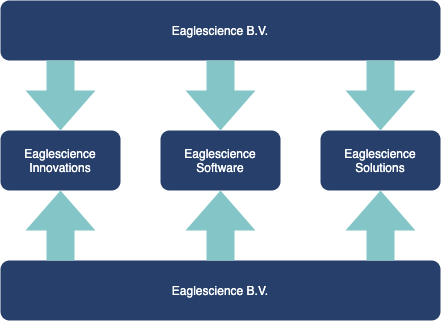
\includegraphics[width=10cm]{gfx/organogram}
\caption{Organogram Eaglescience}
\label{fig:Eaglescience organogram}
\end{figure}
De divisie Eaglescience Innovations zoekt naar nieuwe oplossingen op het gebied van softwareontwikkeling, deze worden door de divisie Eaglescience software geïmplementeerd. Eaglescience Solutions is een divisie die samen met de klant op zoek gaat naar een oplossing voor een gesteld probleem. \\
Het dagelijks bestuur is handen van:
\begin{itemize}
\item CEO / CFO - Marc Grootjen
\item CTO - Bas Breier
\item COO - Wender van Mansvelt
\end{itemize}
Onder het dagelijks bestuur valt Team Eaglescience wat bestaat uit projectmanagers en ontwikkelaars. Deze zijn onderverdeeld in diverse scrum teams die ieders verantwoordelijk zijn voor een project. De ontwikkelaars worden parallel ingezet op meerdere projecten om kennisdeling te bevorderen.

\subsection{Missie}\label{subsec:missie}\marginpar{Missie}

De missie van Eaglescience is het bedienen van haar partners door een ontwerp, ontwikkeling en service te bieden op het gebied van op maat gemaakte IT-oplossingen. Om hier voor te zorgen heeft Eaglescience goed opgeleide IT-professionals in dienst die zichzelf continue ontwikkelen op de “cutting edge” van IT-technologie. De hoofdcompetenties van de medewerkers zijn: innovatief, intelligent, klant georiënteerd, flexibel en ambitieus.

\subsection{Visie}\label{subsec:visie}\marginpar{Visie}
Eaglescience streeft er als innovatief IT-bedrijf naar om software te ontwikkelen als een Business-to-Business dienst. Middels technische vaardigheden bouwen we veilige en hoogwaardige software die bijdraagt aan een betere wereld. Omdat we agile werken, leveren we precies wat nodig is, niets meer en niets minder. Wij helpen onze klanten zoeken naar een langdurige betrokkenheid en samenwerking op basis van zowel vertrouwen als wederzijds respect. \\

Omdat elke vraag uniek is, ontwikkeld Eaglescience op maat gemaakte en innovatieve software.  We zijn van plan deel uit te maken van het hele proces van het formuleren van een idee tot het lanceren van het product en het waarborgen van de productie levenscyclus. Onze belangrijkste succesfactor zijn de mensen, die zich continu ontwikkelen door met de nieuwste technieken te werken op diverse projecten. Wij streven naar een optimale balans tussen werk en privé. Dit geeft onze medewerkers veel vrijheid, maar vereist zelfdiscipline en verantwoordelijkheid.

\subsection{Strategie}\label{subsec:strategie}
\marginpar{strategische thema's}
Eaglescience levert de visie via vier strategische thema's:
\begin{itemize}
    \item Maatschappelijke verantwoordelijkheid
    \item Persoonlijke groei
    \item Tevredenheid
    \item 4e %TODO:Wender vragen
\end{itemize}
We streven ernaar om veilige en hoogwaardige software diensten te leveren die waarde toevoegen aan onze samenleving. We streven naar een bedrijfscultuur waarin alle collega's hun talenten kunnen laten groeien. We hebben een ongecompliceerd werkethos: we richten ons op resultaten van hoge kwaliteit, maar met een gezonde balans tussen werk en privé en voldoende tijd voor leuke en sociale evenementen. Eaglescience verwacht van alle medewerkers dat zij hun handelen baseren op vier kwaliteitsprincipes:
\begin{itemize}
    \item Meld situaties die niet voldoen aan onze interne procedures
    \item Evalueer risico's wanneer grote veranderingen worden verwacht
    \item Help en daag elkaar uit
    \item Kennis behouden over compliancy en kwaliteitsmanagement
\end{itemize}

\section{Werkwijze}\label{sec:werkwijze}
\marginpar{Werkwijze}
Zoals eerder gemeld werkt Eaglescience op projectbasis met ontwikkelaars in meerdere teams. Er wordt geprobeerd "Full scrum" te werken waarbij de requirements van de klant centraal staan. Als een project wordt aangenomen door het managementteam dan wordt deze in sprints in samenspraak met de klant ontwikkeld. De klant wordt nauw betrokken bij het verloop van de ontwikkeling door het geven van demo's aan het einde van iedere sprint. Hier wordt gemeten hoe de applicatie zich gedraagt met betrekking tot de requirements van de klant. Dit is ook het moment dat er feedback gegeven wordt en waar nodig gestuurd kan worden in het verdere verloop. Op het moment dat er een applicatie klaar is wordt de software al dan niet overgedragen aan de klant of doorgegeven aan support en hosting die verantwoordelijk zijn voor de daadwerkelijke hosting van de software.

%TODO: Figuur in NL vertalen
\begin{figure}[bth]
\myfloatalign
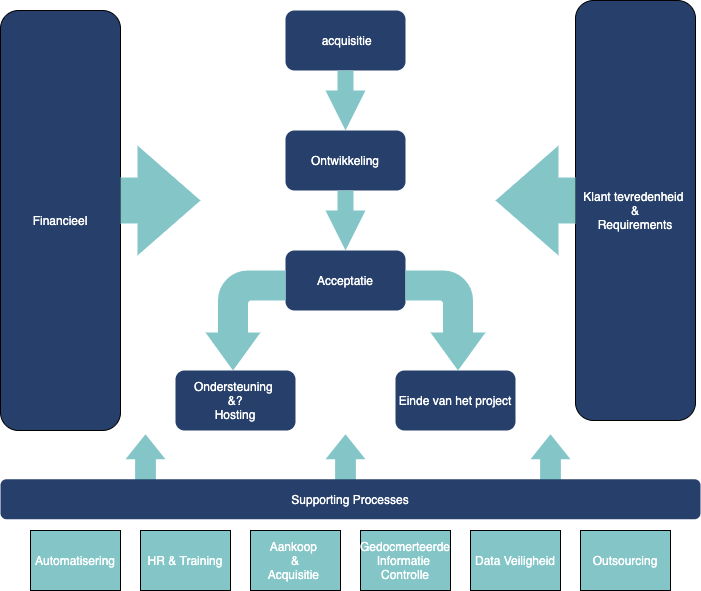
\includegraphics[width=10cm]{gfx/ProcessFlow}
\caption{Project Process}
\label{fig:Project Process}
\end{figure}

Naast het ontwikkel process zijn er een aantal supporting processen die ervoor zorg dragen dat het bedrijf blijft draaien en er nieuwe mensen aangenomen kunnen worden. Maar ook een deel automatisering die voor ondersteuning zorgt van platformen waarop ontwikkeld en/of gehosted wordt.  Eaglescience ontwikkeld op projectbasis en op die manier worden er ook inkomsten gegenereerd. Alle processen die draaien moeten dus ingezet kunnen worden op projecten van klanten. Als er een project voor in huis gebruik wordt ondernomen moet er een duidelijk beeld zijn of er op termijn winst mee te behalen is op monetair vlak dan al niet tijdswinst of ontwikkel gemak.

\section{Relevante en actuele ontwikkelingen binnen Eaglescience}\label{sec:relevante-en-actuele-ontwikkelingen-binnen-eaglescience}
\marginpar{actuele ontwikkelingen}
Eaglescience is aan het groeien, zowel in het aantal projecten waar aan gewerkt wordt als het aantal medewerkers. Daarnaast worden de diensten die Eaglescience aanbied ook uitgebreid, en wordt het hosten van de ontwikkelde applicaties steeds vaker aangeboden. Door deze inzet ligt de verantwoordelijkheid niet alleen bij het leveren van een veilige en hoogwaardige software, maar ook bij het leveren van een veilige hosting service. Naast de groei van het bedrijf is ook zeker de uitbreiding van diensten die aangeboden worden een reden om taken die geautomatiseerd kunnen dan ook te automatiseren.
